% one-figure manuscript written by fig_qc.py --tek-sekil-tex (trap T29)
\begin{figure*}[!t]
\centering
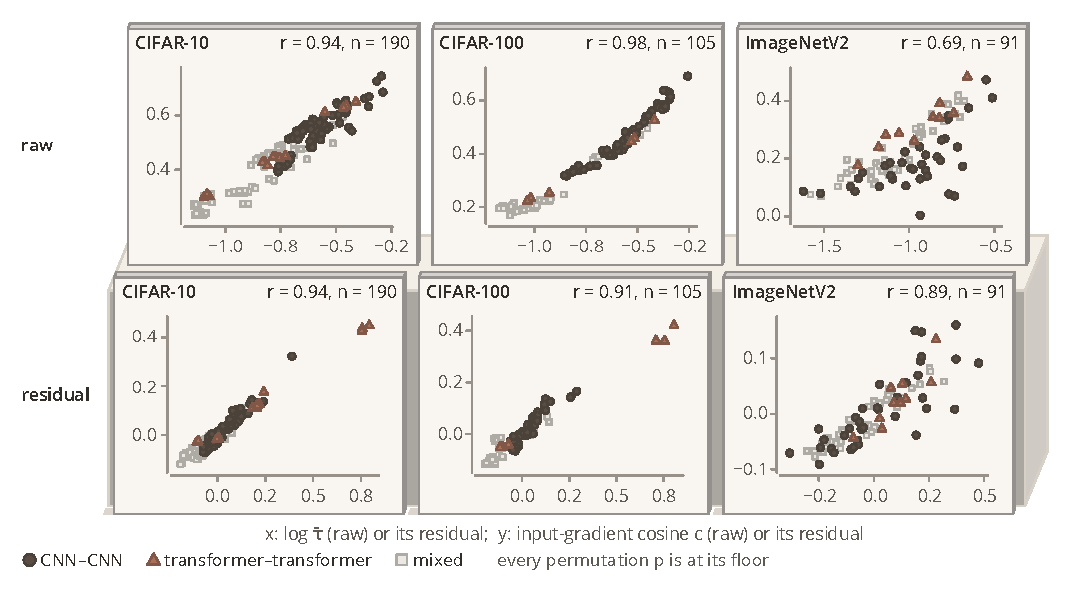
\includegraphics{fig11_gradient_alignment}
\caption{\textbf{Input-gradient alignment against similarity on three steles.} Cosine c between input gradients against log τ̄ for every model pair on CIFAR-10, CIFAR-100 and ImageNetV2; upper panels raw, lower panels residual below the ledge, with additive model main effects removed. Each panel prints the Spearman r and pair count n; values are positions on the flat faces.}
\label{fig:fig11_gradient_alignment}
\end{figure*}
